\section{Feature-first block model}

In this section we propose a novel generative model for modelling labelled networks. We restrict our analysis to labelled, undirected graphs with $N$ nodes. We define the vector $x_i \in \Xcal^D$ as the feature vector for the $i$'th vertex. Each vertex has $D$ total features and we assume all entries take values from the same set $\Xcal$. For the majority of datasets we analyse, we deal with binary feature flags so $\Xcal = \{0, 1\}$. The feature vectors $\{x_i\}_{i=1}^{N}$ are subsumed into the $N \times D$ matrix $X$.

The proposed generative model (which we call the feature-first block model - FFBM) is given in figure \ref{fig:ffbm}. We start, with the feature matrix X and generate a vector of block memberships $b$. The parameters of this step are encapsulated by $\theta$. Each feature vector $x_i$ is treated independently and used to generate the block membership $b_i$. Each entry $b_i \in \{1, 2 \dots B\}$ where $B$ is the number of blocks and a constant in our model. We choose a single softmax layer to model $p(b_i | x_i, \theta)$. More complex models are possible but then deriving meaning from inferred parameter distributions is more difficult. Summarising, we write $p(b | X, \theta)$ as follows:
%
\begin{equation}
	p(b| X, \theta) = \prod_{i=1}^{N} p(b_i | x_i, \theta) = \prod_{i=1}^{N} \phi_{b_i} (x_i; \theta)
	= \prod_{i=1}^{N} \frac{\exp\left(w_{b_i}^T \tilde{x}_i\right)}{\sum_{k=1}^{B} \exp \left( w_k^T \tilde{x}_i\right)}
\end{equation}
%
Where $\tilde{x} \coloneqq \left[x_1, x_2, \dots x_D, 1\right]^T$ is an augmented version of $x$ that allows for a bias term. The parameters for this stage are denoted $\theta$ and consist of the all $B$ weight vectors $\theta = \{w_k\}_{k=1}^{B}$. Each $w_k$ has dimension $D+1$. We could instead write the parameters $\theta$ as a $B \times (D+1)$ matrix of weights $W$; this form has use computationally as then $Z_i = W \tilde{x}_i$ is the input to the softmax activation function.

\begin{figure}[!h]
	\centering
	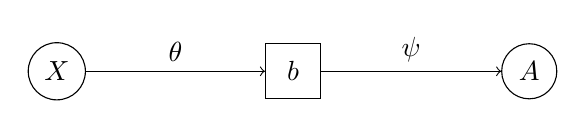
\begin{tikzpicture}[
		roundnode/.style={circle, draw=black, minimum size=7mm},
		squarednode/.style={rectangle, draw=black, minimum size=7mm}
		]
		% nodes
		\node[roundnode] (X) at (0, 0) {$X$};
		\node[squarednode] (b) at (3, 0) {$b$};
		\node[roundnode] (A) at (6, 0) {$A$};
		
		% arrows
		\draw[->] (X.east) -- node[above] {$\theta$} (b.west);
		\draw[->] (b.east) -- node[above] {$\psi$}(A.west);
	\end{tikzpicture}
	\caption{Feature-first block model}
	\label{fig:ffbm}
\end{figure}

With the block memberships $b$ generated, we then draw the graph $A$ from the microcanical DC-SBM (\ref{defn:microcan-dc-sbm}) with additional parameters $\psi = \{e, k\}$. In a slight abuse of notation we denote the inter-block edge count matrix with $e = \psi_e$ and the degree sequence $k = \psi_k$ to make explicit that these parameters are contained in $\psi$.
%
\begin{equation}
	A \sim \textrm{DC-SBM}_{\textrm{MC}} (b, \psi_e, \psi_k)
\end{equation}


\subsection{Prior selection}

Before performing any inference, we must specify priors on $\theta$ and $\psi$. For $\theta$ it seems sensible to choose a Gaussian prior, with zero mean and variance matrix $\sigma^2_\theta I$ such that each element of $\theta$ is independent and distributed like $\sim \Gaussian(0, \sigma_\theta^2)$. In vector form, the prior for $\theta$ is therefore:
%
\begin{equation}
	p(\theta) = \Gaussian \left( \theta ; 0, \sigma_\theta^2 I \right)
	\label{eqn:theta-prior}
\end{equation}
%
We will see that this form of prior is equivalent to a regularisation term in neural network training that penalises extreme weight magnitudes. For $\sigma_\theta^2 \rightarrow \infty$ this becomes an uninformative uniform prior.

In our model, the block memberships vector $b$ is an intermediate latent variable and so we are not free to choose a prior for it. Nevertheless, as far as inference on the right-hand-side of figure \ref{fig:ffbm}, we regard $p(b | X)$ as a pseudo-prior on $b$. We can show (appendix \ref{appdx:b|x}) that our choice of prior for $p(\theta)$ in equation \ref{eqn:theta-prior} leads to a uniform $p(b | X)$ in equation \ref{eqn:b-pseudo-prior}.
%
\begin{equation}
	p(b | X) = \int p(b | X, \theta) p(\theta) d\theta = B^{-N}
	\label{eqn:b-pseudo-prior}
\end{equation}
%
This is a uniform distribution that only depends on the number of blocks $B$. This simplifies the problem nicely as evaluating $p(b | X)$ does not require knowing the exact value $X$ takes. \citet{Peixoto-Bayesian-Microcanonical} proposes careful choices for the additional microcanonical SBM parameters $\psi$ which we adopt. Peixoto's idea is to write the joint prior on $(b, e, k)$ as a product of conditionals $p(b, e, k) = p(b) p(e | b) p(k | e, b)= p(b) p(\psi | b)$. For our purposes we must insert a conditioning on $X$, to form our pseudo-prior for $b$ and $\psi$, to give equation \ref{eqn:joint-pseudo-prior}.
%
\begin{equation}
	p(b, \psi | X) = p(b | X) p(\psi | b, X) = p(b | X) p(\psi | b)
	\label{eqn:joint-pseudo-prior}
\end{equation}
%
Where the simplification is made apparent by noting $(\psi \indep X) | b$. We then borrow the priors proposed by \citet{Peixoto-Bayesian-Microcanonical} for $p(\psi | b)$, repeated here for reference.
%
\begin{equation}
	p(\psi | b) = p(e | b) p(k | e, b) = \left[ \specialchoose{ \specialchoose{B}{2} }{ E} \right]^{-1} 
	\cdot \left[ \prod_r \frac{\prod_j \eta_j^r !}{n_r! q(e_r, n_r)} \right]
\end{equation}
%
Where $\specialchoose{n}{m}$ is shorthand for $\binom{n+m-1}{m} = \frac{(n+m-1)!}{(n-1)!(m)!}$ which can be thought of as the total number of distinct histograms with $n$ bins under the constraint they sum to $m$. $E = \frac{1}{2} \sum_{r,s} e_{rs}$ is the total number of edges in the graph. Importantly, $E$ is not allowed to vary and so $p(e|b)$ is uniform with respect to $e$. The variable $\eta_j^r$ is introduced to denote the number of vertices in block $r$ that have degree $j$. Formally, $\eta_j^r \coloneqq \sum_{i} \one\left\{b_i = r \right\} \one \left\{k_i = j \right\}$. Furthermore, $q(m, n)$ is the number of different histograms with at most $n$ non-zero bins that sum to $m$. $q(m, n)$ is related to but different from $\specialchoose{n}{m}$. Lastly, $e_r \coloneqq \sum_{s} e_{rs}$ is the total number of half edges in block r and $n_r \coloneqq \sum_{i} \one\{b_i = r\}$ is the number of vertices assigned to block $r$. Importantly, we have computable forms for $p(\theta)$ and $p(b, \psi | X)$ which will be useful for performing inference.
